% !TEX root = ../../main.tex


\begin{figure}[!htb]
\centering
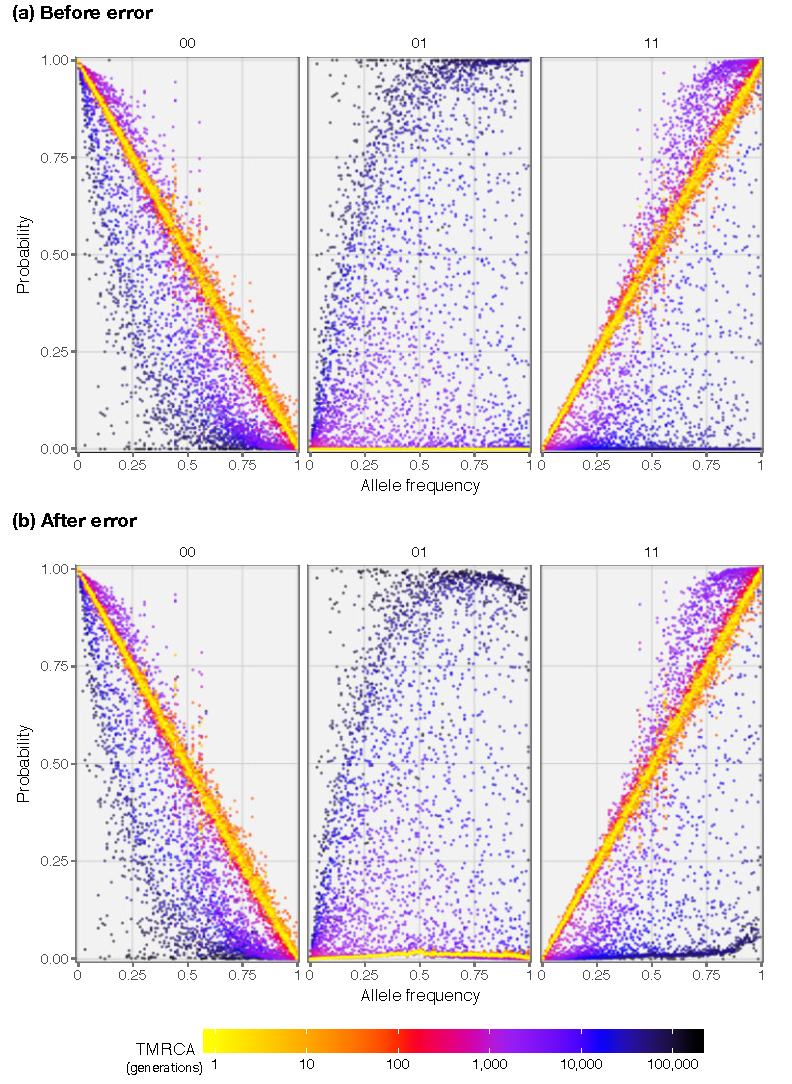
\includegraphics[width=0.75\textwidth]{./img/ch5/hhmm_emission_tmrca_lowres}
\Caption{Empirical probability to observe allelic pairs dependent on T\textsubscript{MRCA}}
{Using data before and after error (datasets $\mathcal{D}_B$ and $\mathcal{D}_B^{\ast}$), the rate at which the possible allelic pairs $(0,0)$, $(0,1)$, and $(1,1)$ were observed is shown by allele frequency, distinguished by the \gls{tmrca} between two haplotypes at a given site.
Empirical observation rates were measured at \n{100000} randomly selected haplotype pairs.
The resulting rates were averaged over \n{100} equally sized allele frequency bins and \n{100} time intervals of equal size on log-scale.
Panels \textbf{(a)} and \textbf{(b)} show the empirical distribution before and after error, respectively.}
{fig:hhmm_emission_trmca}
\end{figure}
